\section{AWS IoT Greengrass / Edge Node Deployment}
\subsection{Extract, Transform and Load Testing}
The testing of the localised Lambda funcitons were completed individually one function at a time. As each Lambda function sends MQQT messages to the IoT Cloud via various subscriptions and topics, these were monitored to see correct functionality of the function. These topics and subscriptions were all discussed in the previous sections and are seen more specifically within Figure \ref{fig:mqqt_testing_setup}
\subsubsection{Extract Lambda Function}
There are three topics that the extract function outputs onto:
\begin{itemize}
    \item extract/checkFile
    \item extract/json
    \item transform/ready
\end{itemize}
The, first item is the \textit{extract/checkFile} which is constantly looking for a .db file placed into the shared directory between the Edge Node and the connected User-Endpoint to the wireless access point.  These output messages can be seen in Figure \ref{fig:extract_checkFile}. Initially no .db file is seen. Upon a .db file being placed into the shared directory, the extract function opens the file and then confirms it is able to open it.

\begin{figure}[ht]
    \centering
    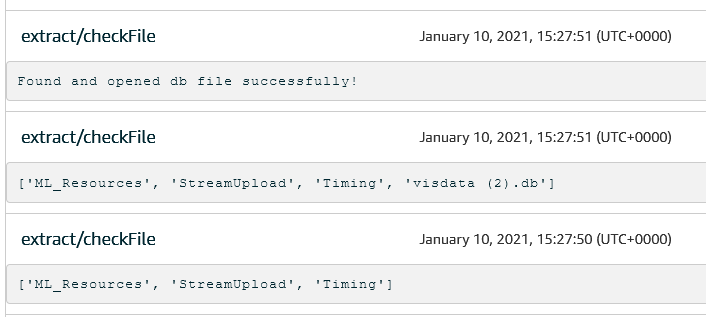
\includegraphics[width=1\linewidth]{pages/Chapter5/Chapter 5 images/Lambda-Fns/extract_checkFile.png}
    \caption{Output of MQQT Packets sent to IoT Cloud from the Extract Lambda Function}
    \label{fig:extract_checkFile}
\end{figure}

The second item is the \textit{extract/json}, which is the timing taken for each data table to be extracted from the .db file. As these are completed, they are assembled into a JSON object and published to the topic. The output of this is similar to the messages sent to the Web Application as the timing data is contained within as seen in Figure \ref{fig:extract_json}.

\begin{figure}[ht]
    \centering
    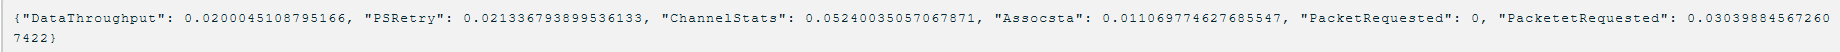
\includegraphics[width=1\linewidth]{pages/Chapter5/Chapter 5 images/Lambda-Fns/extract_json.png}
    \caption{Output of Extraction of JSON Files from Data-table from the .db File}
    \label{fig:extract_json}
\end{figure}

The extract-function then sends the current time that the output file was generated, this time also happens to be pre-pended onto the output JSON files, hence is needed by the transform function to open the newly generated files correctly. This message from one Lambda function to another is seen in Figure \ref{fig:transform_ready}.

\begin{figure}[ht]
    \centering
    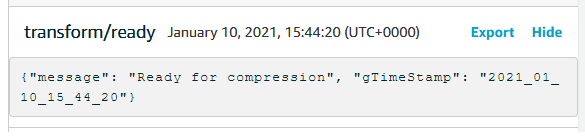
\includegraphics[width=0.7\linewidth]{pages/Chapter5/Chapter 5 images/Lambda-Fns/transform_ready.png}
    \caption{Telling the Transform function to wake and the name of the files to be opened.}
    \label{fig:transform_ready}
\end{figure}

\subsubsection{Transform Lambda Function}
The transform function sends out two MQQT packages under the topics of:
\begin{itemize}
    \item transform/load
    \item transform/extract
\end{itemize}

Once the data within \textit{transform/ready} is sent, and more specifically the \textit{TimeStamp} data, which contains a string that the new 5 generated files begin with, the transform function can begin its correct operation. As it can be seen in Figure \ref{fig:transform_load}, each of the 5 JSON file names begin with the name given in the \textit{gTimeStamp} value. This would not be possible as the timestamp changes from every new db file inserted into the shared folder. After each JSON file is uploaded, a \textit{Succesfully Load JSON files} message is provided to indicate files were all succesfully found. These load messages are sent along the \textit{transform/load} topic.

\begin{figure}[ht]
    \centering
    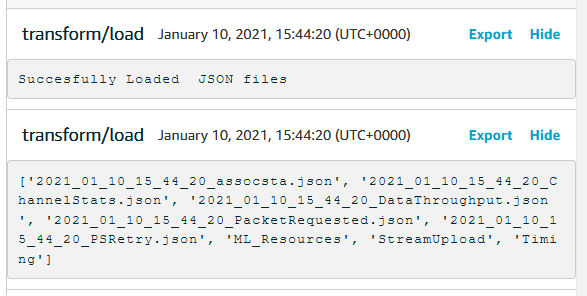
\includegraphics[width=0.7\linewidth]{pages/Chapter5/Chapter 5 images/Lambda-Fns/transform_load.png}
    \caption{Transform function loads the 5 JSON files}
    \label{fig:transform_load}
\end{figure}

Upon loading of the files, data must then be extracted and compressed to a single JSON file. A short and curt message here is enough to indicate the process has been completed and the new JSON file has been stored into all three new locations, for the Load, Local-ML and Remote-ML functions, and is sent across the \textit{transform/extract} topic.

\begin{figure}[ht]
    \centering
    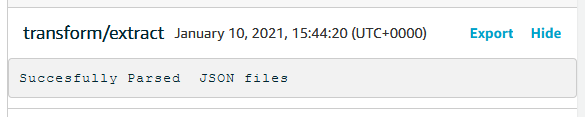
\includegraphics[width=0.5\linewidth]{pages/Chapter5/Chapter 5 images/Lambda-Fns/transform_extract.png}
    \caption{Tranform Function has completed its compression and saving tasks for these 5 new JSON files}
    \label{fig:my_label}
\end{figure}

\subsubsection{Load Lambda Function}
From this Lambda function, the compressed JSON file is uploaded to S3 for storage and any long term analysis. The main topics for testing purposes that this Lambda function is subscribed to are as follows:
\begin{itemize}
    \item load/checkFile
    \item load/uploadFile
\end{itemize}

This Lambda function has a basic task, but first must load the JSON file into the program. This is done by continually checking the directory for \textit{/dest/Stream-Upload/...}. If anything is found here, it will load the JSON files found one at a time. The first topic that is published to by the Lambda function, \textit{load/checkFile}, outputs every 5 seconds to what files it can see in the directory it searches in for JSON files. Upon finding a JSON file, it loads that specific JSON file and this is seen in Figure \ref{fig:load_checkFile}. The lowest message shows an empty directory, then after 5 seconds it is checked again and a new JSON file is found and is then loaded and shown to be loaded succesfully.



\begin{figure}[ht]
    \centering
    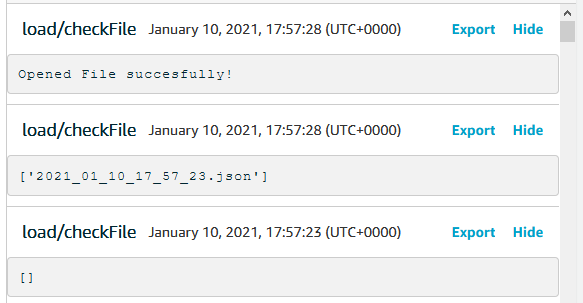
\includegraphics[width=1\linewidth]{pages/Chapter5/Chapter 5 images/Lambda-Fns/load_checkFile.png}
    \caption{MQQT Packets seen after loading JSON file}
    \label{fig:load_checkFile}
\end{figure}

Once the JSON file is loaded and the JSON data is extracted, then a request payload is formed, with the body of the payload as the JSON object as discussed in the designed section and the headers as required for correct authentication to the endpoint. Upon receiving a status code of the 200 after sending the put request, the lambda function will then publish onto the topic, \textit{load/uploadFile} that the function succesfully completed as seen in Figure \ref{fig:load_uploadFile}. 

\begin{figure}[ht]
    \centering
    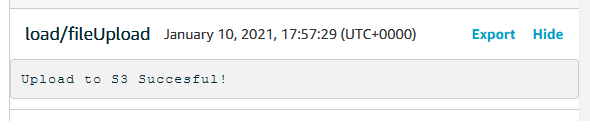
\includegraphics[width=1\linewidth]{pages/Chapter5/Chapter 5 images/Lambda-Fns/load_fileUpload.png}
    \caption{Upon successful upload to S3, this message is sent to the IoT Cloud}
    \label{fig:load_uploadFile}
\end{figure}


\subsubsection{Local-ML Inference Testing}
For the Local-ML Inference testing, the testing method is shown in a different format. The IoT Cloud Method is already shown off, however another method is for the output data and timings to be written to a file. In this output file, data that has been already filtered to fit the model's required input format, timing data and classification by the model is written into the file. Since this model classification and data output must also be verified by other members of the project, it is important to also have this output data stored. An example of one timestamp's set of input data for the model is shown in Figure \ref{fig:local-ml-output}, where the data input set of \textbf{[0,0,0,0,0,1,95]} correctly corresponds to '3.0' or 'Very Weak'. This data output is stored and then transferred for model verification and it also transferred as MQQT Packages to the Web Server for live data viewing. This latter point is discussed further in the Web Application testing.

\begin{figure}[ht]
    \centering
    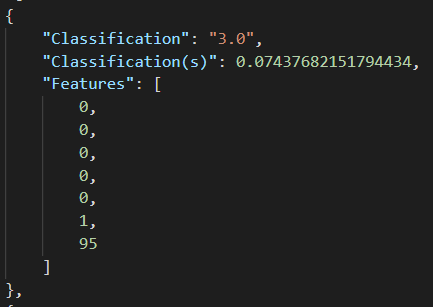
\includegraphics[width=0.5\linewidth]{pages/Chapter5/Chapter 5 images/Lambda-Fns/local_ml_fn_output.png}
    \caption{Local Machine Learning Lambda Function's Output Format}
    \label{fig:local-ml-output}
\end{figure}

The output here shows correct operation as is discussed in the ML Sections of the project and how the value of this classification corresponds to the equivalent of 'Very Weak' data throughput.


\subsubsection{Remote-ML Inference Testing}
The Remote-ML Inference testing simply uses an API Endpoint which is tested using Post Man in Section \ref{post_man_testing}. The Lambda function uses the Python requests library to package and sends the JSON data to the Cloud for classification. The response is shown in the mentioned section further in the report. The data received by the post request is then transferred to the Web App directly for live viewing.


\subsection{NodeJS Web Server Application}
The web application is being used for live-data viewing to see data being handled in the back-end and how long it took each Lambda function for processing in the various stages and transfer to the Cloud. For the testing of the NodeJS Web Server Application, all systems were needed to be running. These includes the automatic data retrieval from the SSH; transfer of files from the laptop to the edge node; ETL on the incoming data and then provisioning the ML Model for localised inference of the data throughput based on Channel Stats; ML-inference is also seen by sending the input data parameters to the cloud and getting inference directly from the Sagemaker endpoint. 

\begin{figure}[ht]
    \centering
    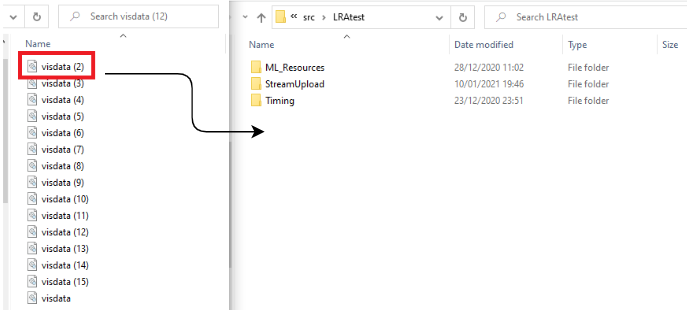
\includegraphics[width=1\linewidth]{pages/Chapter5/Chapter 5 images/testing_node_js_manually.png}
    \caption{Feeding the Edge Node directory }
    \label{fig:feeding_edge_node_manually}
\end{figure}
The first test however, would be to manually feed the edge-node with .db files and seeing the response of the developed Web Application. This method is shown in Figure \ref{fig:feeding_edge_node_manually}. The twelve files are inserted into the shared directory one at a time. As soon as the Edge Node begins processing, data can be seen streaming into the Web Server. In the first image shown in Figure \ref{fig:node_testing_1}, the data can be seen as having been processed by the extract and transform functions. The Load function has not been completed but the ML-Local inference has begun processing. The data throughput and classification data appearing in the table proves this, and as the Local-ML total timing has not yet been shown it can be deduced that the Local-ML is still running. The completed duration to scan and run each file within the Lambda functions is shown on the right. The remote, cloud-based ML Model is unreachable and goes to prove why deploying models to local environments is so useful in this testing example.
\begin{figure}[ht]
    \centering
    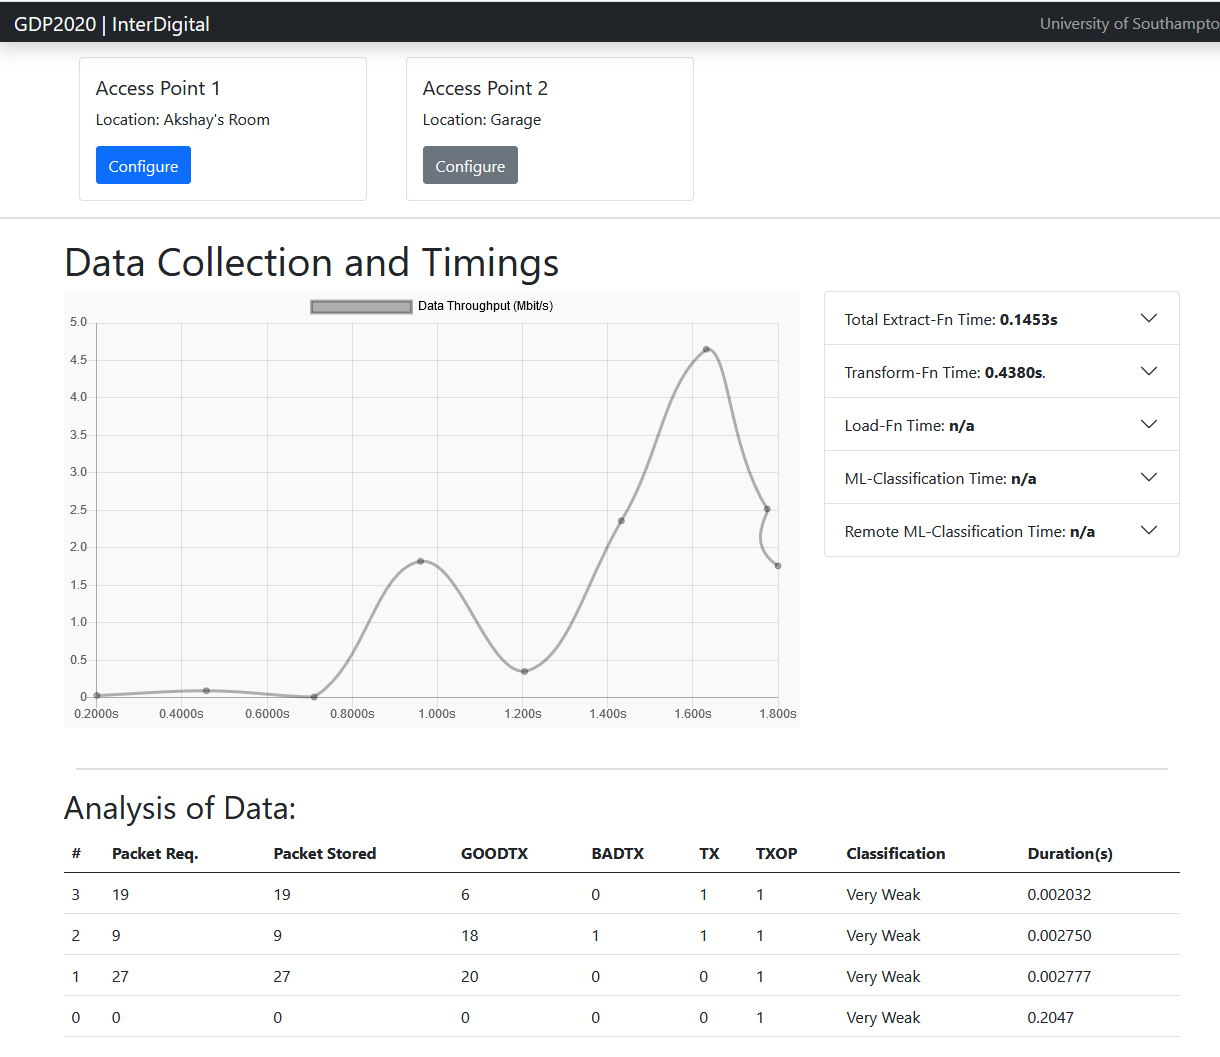
\includegraphics[width=1\linewidth]{pages/Chapter5/Chapter 5 images/testing_pt1.png}
    \caption{Data has been processed by Extract and Transform Lambda functions, and is still being processed by Load and Local-ML Lambda functions}
    \label{fig:node_testing_1}
\end{figure}

The final live-data view for one .db file is seen in Figure \ref{fig:node_testing_2}.A few key timings can be seen:
\begin{itemize}
    \item Extraction from .db File: \textbf{0.15s}
    \item Transformation time to compress into a single JSON file: \textbf{0.44s}
    \item Load time of compressed JSON to S3: \textbf{1.743s}
    \item Local-ML classificaiton of the whole file: \textbf{0.58s}
    \item Remote-ML Classification time: \textbf{n/a}
\end{itemize}
A full comparison between Local-ML and Remote-ML will be shown in the Results section, but correct operation of the NodeJS Web application was shown and therefore can be used for testing and validation of the deployed model.
\begin{figure}[ht]
    \centering
    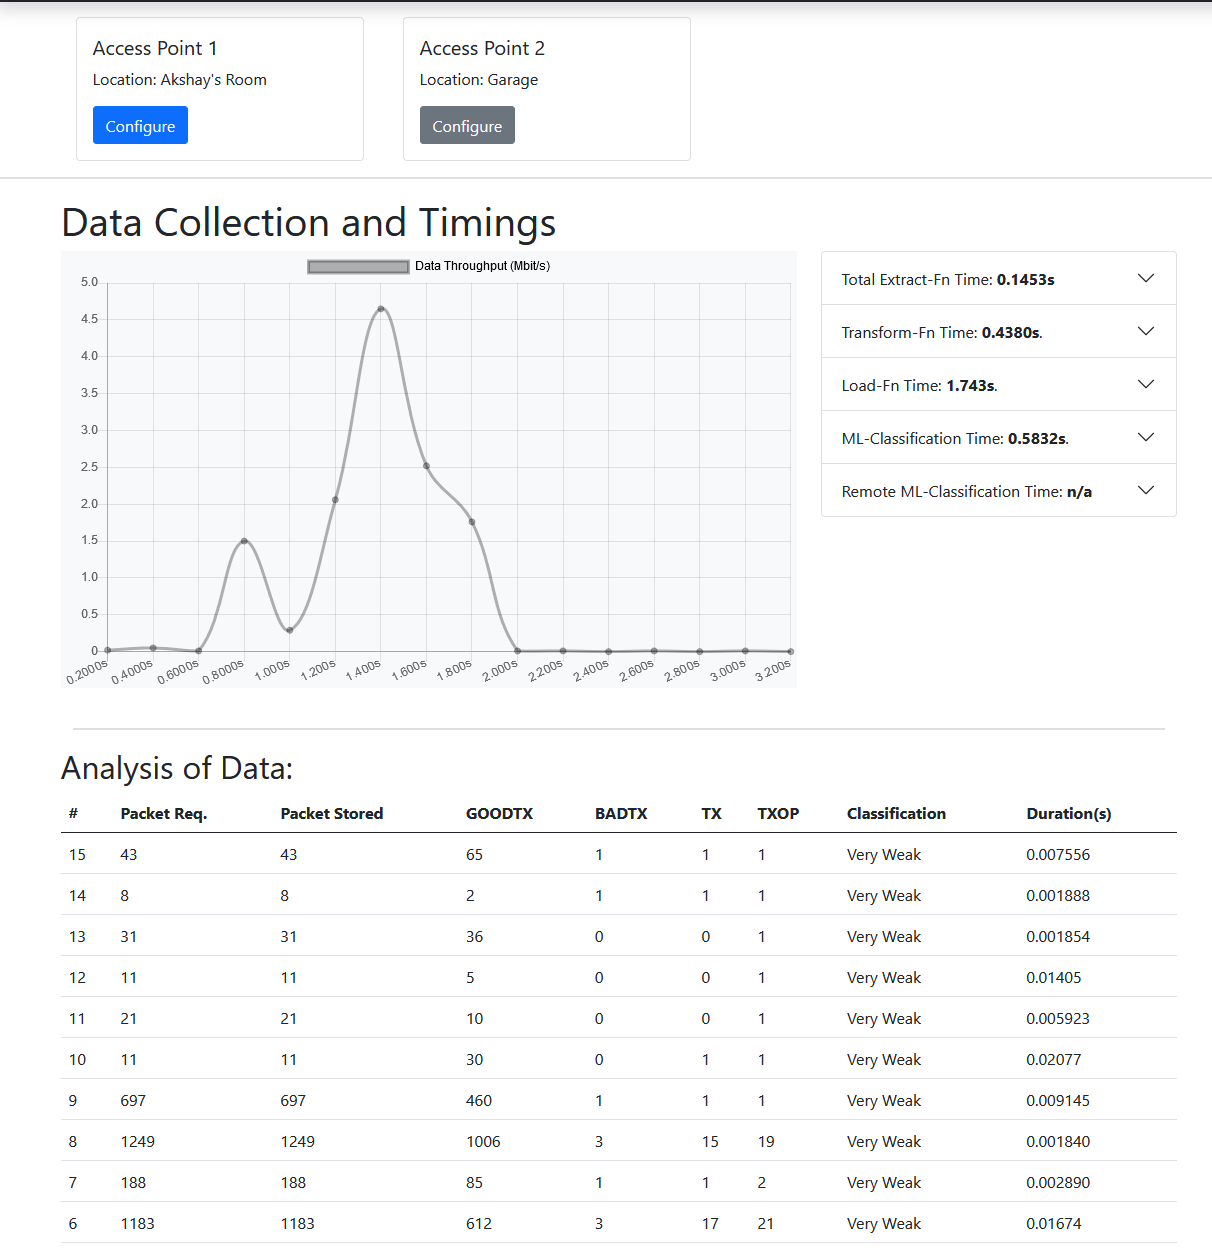
\includegraphics[width=1\linewidth]{pages/Chapter5/Chapter 5 images/testing_pt2.png}
    \caption{Full testing with Manual .db File Placement.}
    \label{fig:node_testing_2}
\end{figure}
